\chapter{Clustered MGXS Model Verification}
\label{chap:results}


%%%%%%%%%%%%%%%%%%%%%%%%%%%%%%%%%%%%%%%%%%%%%%%%%%%%%%%%%%%%%%%%%%%%%%%%%%%%%%%
\section{Verification Metrics}
\label{sec:chap7-verify}


%%%%%%%%%%%%%%%%%%%%%%%%%%%%%%%%%%%%%%%%%%%%%%%%%%%%%%%%%%%%%%%%%%%%%%%%%%%%%%%
\section{Model Evaluation}
\label{sec:chap7-evaluate}

\begin{itemize}[noitemsep]
  \item how much ``noise'' can we live with in our tally data???
  \item ``perfect'' clustering
  \item ``adaptive'' clustering
\end{itemize}


%%%%%%%%%%%%%%%%%%%%%%%%%%%%%%%%%%%%%%%%%%%%%%%%%%%%%%%%%%%%%%%%%%%%%%%%%%%%%%%
\section{Performance with Converged MGXS}
\label{sec:chap11-improvements}

%%%%%%%%%%%%%%%%%%%%%%%%%%%%
\subsection{Eigenvalue Bias}
\label{subsec:chap11-eigenvalue-bias}


\begin{table}[ht!]
  \centering
  \caption[OpenMOC eigenvalue bias for null feature selection]{OpenMOC eigenvalue bias $\Delta\rho$ for null feature selection for \textit{i}\ac{MGXS} spatial homogenization with varying clustering algorithms.}
  \small
  \label{table:chap11-eigenvalues-combined}
  \vspace{6pt}
  \begin{tabular}{l l R{1.5cm} R{1.5cm} R{1.5cm} R{1.5cm} R{1.5cm}}
  \toprule
  \rowcolor{lightgray}
  & \multicolumn{1}{c}{\cellcolor{lightgray} \bf Clustering} & \multicolumn{5}{S[table-format=6.1]}{\cellcolor{lightgray} \textbf{\# Clusters}} \\
  \multirow{-2}{*}{\cellcolor{lightgray} \bf Benchmark} &
  \multicolumn{1}{c}{\cellcolor{lightgray} \bf Algorithm} &
  \multicolumn{1}{c}{\cellcolor{lightgray} \bf 2} &
  \multicolumn{1}{c}{\cellcolor{lightgray} \bf 4} &
  \multicolumn{1}{c}{\cellcolor{lightgray} \bf 6} &
  \multicolumn{1}{c}{\cellcolor{lightgray} \bf 8} &
  \multicolumn{1}{c}{\cellcolor{lightgray} \bf 10} \\
  \midrule
\multirow{4}{*}{\parbox{2.5cm}{1.6\% Assm}} & $k$-Means & & & & & \\
& Agglomerative & & & & & \\
& BIRCH & & & & & \\
& GMM & & & & & \\
  \midrule
\multirow{4}{*}{\parbox{2.5cm}{3.1\% Assm}} & $k$-Means & & & & & \\
& Agglomerative & & & & & \\
& BIRCH & & & & & \\
& GMM & & & & & \\
  \midrule
\multirow{4}{*}{\parbox{2.5cm}{3.1\% Assm w/ 20 BPs}} & $k$-Means & & & & & \\
& Agglomerative & & & & & \\
& BIRCH & & & & & \\
& GMM & & & & & \\
  \midrule
\multirow{4}{*}{\parbox{2.5cm}{2$\times$2 Colorset}} & $k$-Means & & & & & \\
& Agglomerative & & & & & \\
& BIRCH & & & & & \\
& GMM & & & & & \\
  \midrule
\multirow{4}{*}{\parbox{2.5cm}{2$\times$2 Colorset w/ Reflector}} & $k$-Means & & & & & \\
& Agglomerative & & & & & \\
& BIRCH & & & & & \\
& GMM & & & & & \\
  \midrule
\multirow{4}{*}{\parbox{2.5cm}{BEAVRS Full Core}} & $k$-Means & & & & & \\
& Agglomerative & & & & & \\
& BIRCH & & & & & \\
& GMM & & & & & \\
  \bottomrule
\end{tabular}
\end{table}

\clearpage

\begin{table}[ht!]
  \centering
  \caption[OpenMOC eigenvalue bias for pinch feature selection]{OpenMOC eigenvalue bias $\Delta\rho$ for pinch feature selection for \textit{i}\ac{MGXS} spatial homogenization with varying clustering algorithms.}
  \small
  \label{table:chap11-eigenvalues-pinch}
  \vspace{6pt}
  \begin{tabular}{l l R{1.5cm} R{1.5cm} R{1.5cm} R{1.5cm} R{1.5cm}}
  \toprule
  \rowcolor{lightgray}
  & \multicolumn{1}{c}{\cellcolor{lightgray} \bf Clustering} & \multicolumn{5}{S[table-format=6.1]}{\cellcolor{lightgray} \textbf{\# Clusters}} \\
  \multirow{-2}{*}{\cellcolor{lightgray} \bf Benchmark} &
  \multicolumn{1}{c}{\cellcolor{lightgray} \bf Algorithm} &
  \multicolumn{1}{c}{\cellcolor{lightgray} \bf 2} &
  \multicolumn{1}{c}{\cellcolor{lightgray} \bf 4} &
  \multicolumn{1}{c}{\cellcolor{lightgray} \bf 6} &
  \multicolumn{1}{c}{\cellcolor{lightgray} \bf 8} &
  \multicolumn{1}{c}{\cellcolor{lightgray} \bf 10} \\
  \midrule
\multirow{4}{*}{\parbox{2.5cm}{1.6\% Assm}} & $k$-Means & & & & & \\
& Agglomerative & & & & & \\
& BIRCH & & & & & \\
& GMM & & & & & \\
  \midrule
\multirow{4}{*}{\parbox{2.5cm}{3.1\% Assm}} & $k$-Means & & & & & \\
& Agglomerative & & & & & \\
& BIRCH & & & & & \\
& GMM & & & & & \\
  \midrule
\multirow{4}{*}{\parbox{2.5cm}{3.1\% Assm w/ 20 BPs}} & $k$-Means & & & & & \\
& Agglomerative & & & & & \\
& BIRCH & & & & & \\
& GMM & & & & & \\
  \midrule
\multirow{4}{*}{\parbox{2.5cm}{2$\times$2 Colorset}} & $k$-Means & & & & & \\
& Agglomerative & & & & & \\
& BIRCH & & & & & \\
& GMM & & & & & \\
  \midrule
\multirow{4}{*}{\parbox{2.5cm}{2$\times$2 Colorset w/ Reflector}} & $k$-Means & & & & & \\
& Agglomerative & & & & & \\
& BIRCH & & & & & \\
& GMM & & & & & \\
  \midrule
\multirow{4}{*}{\parbox{2.5cm}{BEAVRS Full Core}} & $k$-Means & & & & & \\
& Agglomerative & & & & & \\
& BIRCH & & & & & \\
& GMM & & & & & \\
  \bottomrule
\end{tabular}
\end{table}


%%%%%%%%%%%%%%%%%%%%%%%%%%%%%%%%
\subsection{U-238 Capture Rates}
\label{subsec:chap11-capture-rates}

\begin{itemize}[noitemsep]
  \item bar charts of max/mean errors for varying \# clusters
  \item heat maps of capture rates, errors, improvements
  \item histogram of capture rate errors
\end{itemize}

-put tables for PCA and ensemble transforms in appendix
-need tables for both combined and pinch feature selection

\begin{table}[ht!]
  \centering
  \caption[Mean OpenMOC U-238 capture rate errors for null feature selection]{Mean absolute U-238 capture rate percent relative errors for null feature selection for \textit{i}\ac{MGXS} spatial homogenization with varying clustering algorithms.}
  \small
  \label{table:chap11-max-capt-rates-null}
  \vspace{6pt}
  \begin{tabular}{l l R{1.5cm} R{1.5cm} R{1.5cm} R{1.5cm} R{1.5cm}}
  \toprule
  \rowcolor{lightgray}
  & & \multicolumn{5}{S[table-format=6.1]}{\cellcolor{lightgray} \textbf{\# Clusters}} \\
  \multirow{-2}{*}{\cellcolor{lightgray} \bf Benchmark} &
  \multirow{-2}{*}{\cellcolor{lightgray} \bf Predictor} &
  \multicolumn{1}{c}{\cellcolor{lightgray} \bf 2} &
  \multicolumn{1}{c}{\cellcolor{lightgray} \bf 4} &
  \multicolumn{1}{c}{\cellcolor{lightgray} \bf 6} &
  \multicolumn{1}{c}{\cellcolor{lightgray} \bf 8} &
  \multicolumn{1}{c}{\cellcolor{lightgray} \bf 10} \\
  \midrule
\multirow{4}{*}{\parbox{2.5cm}{1.6\% Assm}} & $k$-Means & & & & & \\
& Agglomerative & & & & & \\
& BIRCH & & & & & \\
& GMM & & & & & \\
  \midrule
\multirow{4}{*}{\parbox{2.5cm}{3.1\% Assm}} & $k$-Means & & & & & \\
& Agglomerative & & & & & \\
& BIRCH & & & & & \\
& GMM & & & & & \\
  \midrule
\multirow{4}{*}{\parbox{2.5cm}{3.1\% Assm w/ 20 BPs}} & $k$-Means & & & & & \\
& Agglomerative & & & & & \\
& BIRCH & & & & & \\
& GMM & & & & & \\
  \midrule
\multirow{4}{*}{\parbox{2.5cm}{2$\times$2 Colorset}} & $k$-Means & & & & & \\
& Agglomerative & & & & & \\
& BIRCH & & & & & \\
& GMM & & & & & \\
  \midrule
\multirow{4}{*}{\parbox{2.5cm}{2$\times$2 Colorset w/ Reflector}} & $k$-Means & & & & & \\
& Agglomerative & & & & & \\
& BIRCH & & & & & \\
& GMM & & & & & \\
  \midrule
\multirow{4}{*}{\parbox{2.5cm}{BEAVRS Full Core}} & $k$-Means & & & & & \\
& Agglomerative & & & & & \\
& BIRCH & & & & & \\
& GMM & & & & & \\
  \bottomrule
\end{tabular}
\end{table}

\clearpage

\begin{table}[ht!]
  \centering
  \caption[Maximum OpenMOC U-238 capture rate errors for null feature selection]{Maximum absolute U-238 capture rate percent relative errors for null feature selection for \textit{i}\ac{MGXS} spatial homogenization with varying clustering algorithms.}
  \small
  \label{table:chap11-mean-capt-rates-null}
  \vspace{6pt}
  \begin{tabular}{l l R{1.5cm} R{1.5cm} R{1.5cm} R{1.5cm} R{1.5cm}}
  \toprule
  \rowcolor{lightgray}
  & & \multicolumn{5}{S[table-format=6.1]}{\cellcolor{lightgray} \textbf{\# Clusters}} \\
  \multirow{-2}{*}{\cellcolor{lightgray} \bf Benchmark} &
  \multirow{-2}{*}{\cellcolor{lightgray} \bf Predictor} &
  \multicolumn{1}{c}{\cellcolor{lightgray} \bf 2} &
  \multicolumn{1}{c}{\cellcolor{lightgray} \bf 4} &
  \multicolumn{1}{c}{\cellcolor{lightgray} \bf 6} &
  \multicolumn{1}{c}{\cellcolor{lightgray} \bf 8} &
  \multicolumn{1}{c}{\cellcolor{lightgray} \bf 10} \\
  \midrule
\multirow{4}{*}{\parbox{2.5cm}{1.6\% Assm}} & $k$-Means & & & & & \\
& Agglomerative & & & & & \\
& BIRCH & & & & & \\
& GMM & & & & & \\
  \midrule
\multirow{4}{*}{\parbox{2.5cm}{3.1\% Assm}} & $k$-Means & & & & & \\
& Agglomerative & & & & & \\
& BIRCH & & & & & \\
& GMM & & & & & \\
  \midrule
\multirow{4}{*}{\parbox{2.5cm}{3.1\% Assm w/ 20 BPs}} & $k$-Means & & & & & \\
& Agglomerative & & & & & \\
& BIRCH & & & & & \\
& GMM & & & & & \\
  \midrule
\multirow{4}{*}{\parbox{2.5cm}{2$\times$2 Colorset}} & $k$-Means & & & & & \\
& Agglomerative & & & & & \\
& BIRCH & & & & & \\
& GMM & & & & & \\
  \midrule
\multirow{4}{*}{\parbox{2.5cm}{2$\times$2 Colorset w/ Reflector}} & $k$-Means & & & & & \\
& Agglomerative & & & & & \\
& BIRCH & & & & & \\
& GMM & & & & & \\
  \midrule
\multirow{4}{*}{\parbox{2.5cm}{BEAVRS Full Core}} & $k$-Means & & & & & \\
& Agglomerative & & & & & \\
& BIRCH & & & & & \\
& GMM & & & & & \\
  \bottomrule
\end{tabular}
\end{table}

\clearpage

\begin{table}[ht!]
  \centering
  \caption[Mean OpenMOC U-238 capture rate errors for pinch feature selection]{Mean absolute U-238 capture rate percent relative errors for pinch feature selection for \textit{i}\ac{MGXS} spatial homogenization with varying clustering algorithms.}
  \small
  \label{table:chap11-max-capt-rates-pinch}
  \vspace{6pt}
  \begin{tabular}{l l R{1.5cm} R{1.5cm} R{1.5cm} R{1.5cm} R{1.5cm}}
  \toprule
  \rowcolor{lightgray}
  & & \multicolumn{5}{S[table-format=6.1]}{\cellcolor{lightgray} \textbf{\# Clusters}} \\
  \multirow{-2}{*}{\cellcolor{lightgray} \bf Benchmark} &
  \multirow{-2}{*}{\cellcolor{lightgray} \bf Predictor} &
  \multicolumn{1}{c}{\cellcolor{lightgray} \bf 2} &
  \multicolumn{1}{c}{\cellcolor{lightgray} \bf 4} &
  \multicolumn{1}{c}{\cellcolor{lightgray} \bf 6} &
  \multicolumn{1}{c}{\cellcolor{lightgray} \bf 8} &
  \multicolumn{1}{c}{\cellcolor{lightgray} \bf 10} \\
  \midrule
\multirow{4}{*}{\parbox{2.5cm}{1.6\% Assm}} & $k$-Means & & & & & \\
& Agglomerative & & & & & \\
& BIRCH & & & & & \\
& GMM & & & & & \\
  \midrule
\multirow{4}{*}{\parbox{2.5cm}{3.1\% Assm}} & $k$-Means & & & & & \\
& Agglomerative & & & & & \\
& BIRCH & & & & & \\
& GMM & & & & & \\
  \midrule
\multirow{4}{*}{\parbox{2.5cm}{3.1\% Assm w/ 20 BPs}} & $k$-Means & & & & & \\
& Agglomerative & & & & & \\
& BIRCH & & & & & \\
& GMM & & & & & \\
  \midrule
\multirow{4}{*}{\parbox{2.5cm}{2$\times$2 Colorset}} & $k$-Means & & & & & \\
& Agglomerative & & & & & \\
& BIRCH & & & & & \\
& GMM & & & & & \\
  \midrule
\multirow{4}{*}{\parbox{2.5cm}{2$\times$2 Colorset w/ Reflector}} & $k$-Means & & & & & \\
& Agglomerative & & & & & \\
& BIRCH & & & & & \\
& GMM & & & & & \\
  \midrule
\multirow{4}{*}{\parbox{2.5cm}{BEAVRS Full Core}} & $k$-Means & & & & & \\
& Agglomerative & & & & & \\
& BIRCH & & & & & \\
& GMM & & & & & \\
  \bottomrule
\end{tabular}
\end{table}

\clearpage

\begin{table}[ht!]
  \centering
  \caption[Maximum OpenMOC U-238 capture rate errors for pinch feature selection]{Maximum absolute U-238 capture rate percent relative errors for pinch feature selection for \textit{i}\ac{MGXS} spatial homogenization with varying clustering algorithms.}
  \small
  \label{table:chap11-mean-capt-rates-pinch}
  \vspace{6pt}
  \begin{tabular}{l l R{1.5cm} R{1.5cm} R{1.5cm} R{1.5cm} R{1.5cm}}
  \toprule
  \rowcolor{lightgray}
  & & \multicolumn{5}{S[table-format=6.1]}{\cellcolor{lightgray} \textbf{\# Clusters}} \\
  \multirow{-2}{*}{\cellcolor{lightgray} \bf Benchmark} &
  \multirow{-2}{*}{\cellcolor{lightgray} \bf Predictor} &
  \multicolumn{1}{c}{\cellcolor{lightgray} \bf 2} &
  \multicolumn{1}{c}{\cellcolor{lightgray} \bf 4} &
  \multicolumn{1}{c}{\cellcolor{lightgray} \bf 6} &
  \multicolumn{1}{c}{\cellcolor{lightgray} \bf 8} &
  \multicolumn{1}{c}{\cellcolor{lightgray} \bf 10} \\
  \midrule
\multirow{4}{*}{\parbox{2.5cm}{1.6\% Assm}} & $k$-Means & & & & & \\
& Agglomerative & & & & & \\
& BIRCH & & & & & \\
& GMM & & & & & \\
  \midrule
\multirow{4}{*}{\parbox{2.5cm}{3.1\% Assm}} & $k$-Means & & & & & \\
& Agglomerative & & & & & \\
& BIRCH & & & & & \\
& GMM & & & & & \\
  \midrule
\multirow{4}{*}{\parbox{2.5cm}{3.1\% Assm w/ 20 BPs}} & $k$-Means & & & & & \\
& Agglomerative & & & & & \\
& BIRCH & & & & & \\
& GMM & & & & & \\
  \midrule
\multirow{4}{*}{\parbox{2.5cm}{2$\times$2 Colorset}} & $k$-Means & & & & & \\
& Agglomerative & & & & & \\
& BIRCH & & & & & \\
& GMM & & & & & \\
  \midrule
\multirow{4}{*}{\parbox{2.5cm}{2$\times$2 Colorset w/ Reflector}} & $k$-Means & & & & & \\
& Agglomerative & & & & & \\
& BIRCH & & & & & \\
& GMM & & & & & \\
  \midrule
\multirow{4}{*}{\parbox{2.5cm}{BEAVRS Full Core}} & $k$-Means & & & & & \\
& Agglomerative & & & & & \\
& BIRCH & & & & & \\
& GMM & & & & & \\
  \bottomrule
\end{tabular}
\end{table}

\clearpage

\begin{figure}[h!]
\centering
\begin{subfigure}{0.45\textwidth}
  \centering
  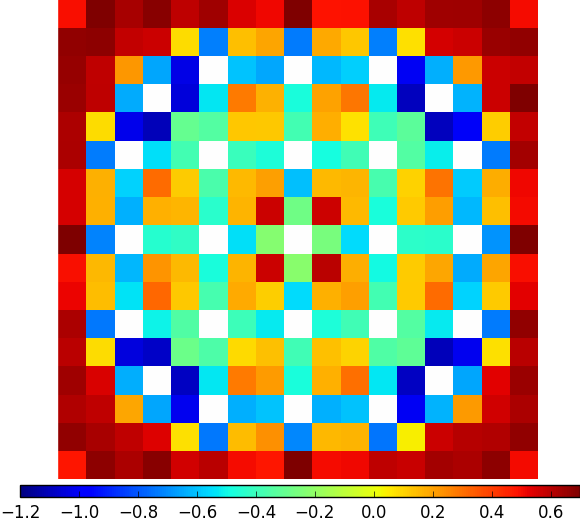
\includegraphics[width=\linewidth]{figures/results/assm-16/no-transform/capt-err-null}
  \caption{}
  \label{fig:chap11-assm-1.6-capt-null}
\end{subfigure}%
\begin{subfigure}{0.45\textwidth}
  \centering
  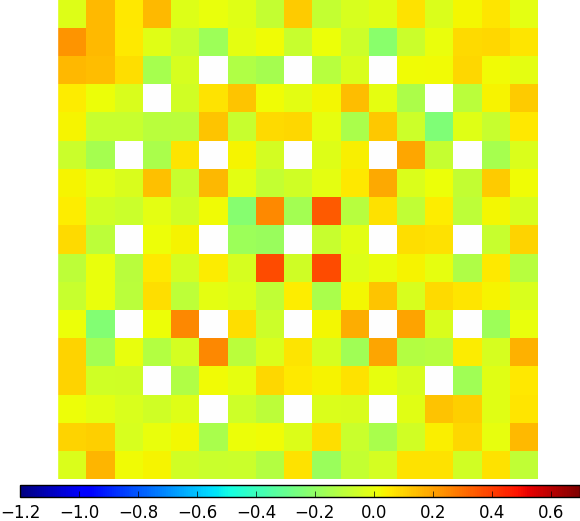
\includegraphics[width=\linewidth]{figures/results/assm-16/no-transform/capt-err-degenerate}
  \caption{}
  \label{fig:chap11-assm-1.6-capt-degenerate}
\end{subfigure}
\begin{subfigure}{0.45\textwidth}
  \centering
  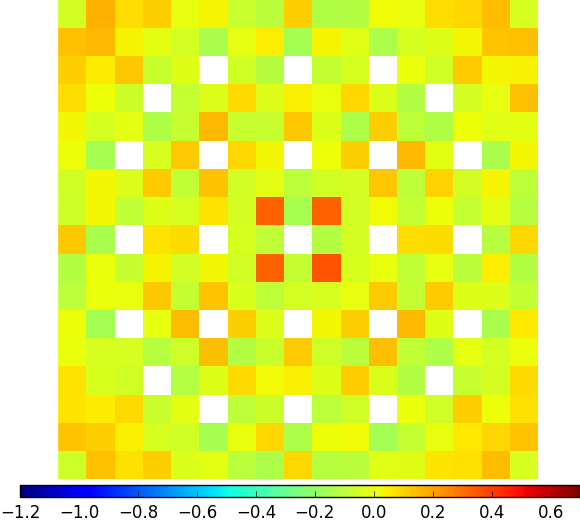
\includegraphics[width=\linewidth]{figures/results/assm-16/no-transform/capt-err-lns}
  \caption{}
  \label{fig:chap11-assm-1.6-capt-lns}
\end{subfigure}%
\begin{subfigure}{0.45\textwidth}
  \centering
  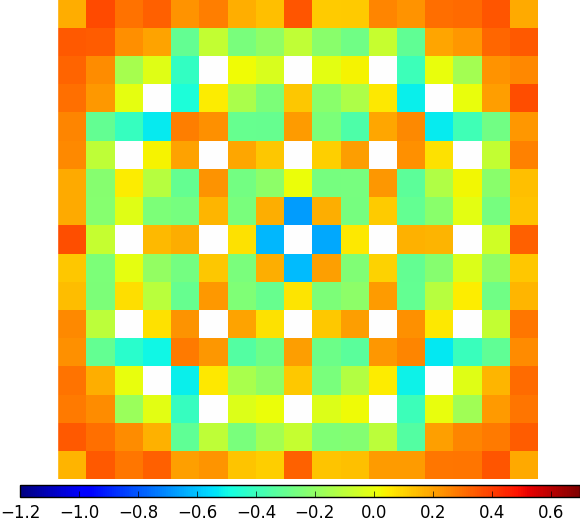
\includegraphics[width=\linewidth]{figures/results/assm-16/no-transform/capt-err-pinch-agglomerative-(2)}
  \caption{}
  \label{fig:chap11-assm-1.6-capt-pinch-2}
\end{subfigure}
\begin{subfigure}{0.45\textwidth}
  \centering
  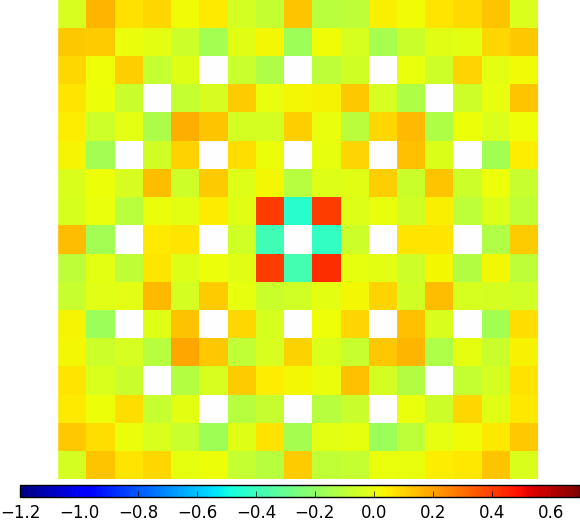
\includegraphics[width=\linewidth]{figures/results/assm-16/no-transform/capt-err-pinch-agglomerative-(6)}
  \caption{}
  \label{fig:chap11-assm-1.6-capt-pinch-6}
\end{subfigure}%
\begin{subfigure}{0.45\textwidth}
  \centering
  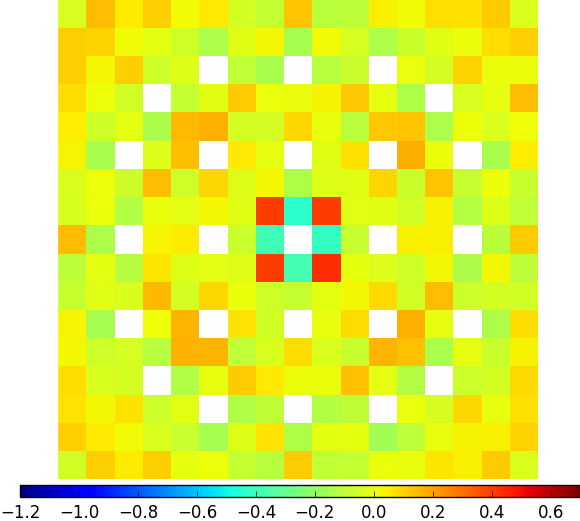
\includegraphics[width=\linewidth]{figures/results/assm-16/no-transform/capt-err-pinch-agglomerative-(10)}
  \caption{}
  \label{fig:chap11-assm-1.6-capt-pinch-10}
\end{subfigure}
\vspace{2mm}
\caption[U-238 capture rate errors for a 1.6\% enriched assembly]{U-238 capture rate error spatial distributions for a 1.6\% enriched assembly for null (a), degenerate (b), \ac{LNS} (c) and \textit{i}\ac{MGXS} spatial homogenization with 2 (d), 6 (e) and 10 (f) clusters.}
\label{fig:chap11-assm-1.6-capt-rates}
\end{figure}

\clearpage

\begin{figure}[h!]
\centering
\begin{subfigure}{0.45\textwidth}
  \centering
  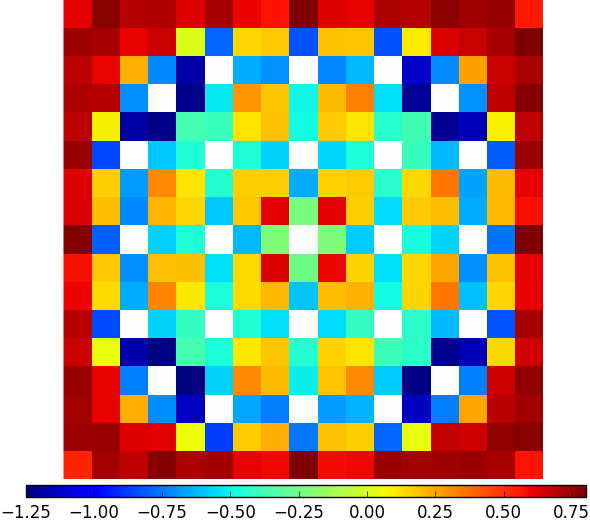
\includegraphics[width=\linewidth]{figures/results/assm-31/pca-transform/capt-err-null}
  \caption{}
  \label{fig:chap11-assm-3.1-capt-null}
\end{subfigure}%
\begin{subfigure}{0.45\textwidth}
  \centering
  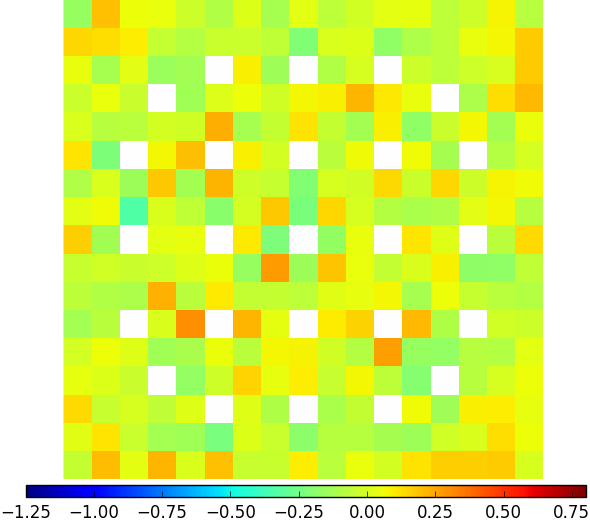
\includegraphics[width=\linewidth]{figures/results/assm-31/pca-transform/capt-err-degenerate}
  \caption{}
  \label{fig:chap11-assm-3.1-capt-degenerate}
\end{subfigure}
\begin{subfigure}{0.45\textwidth}
  \centering
  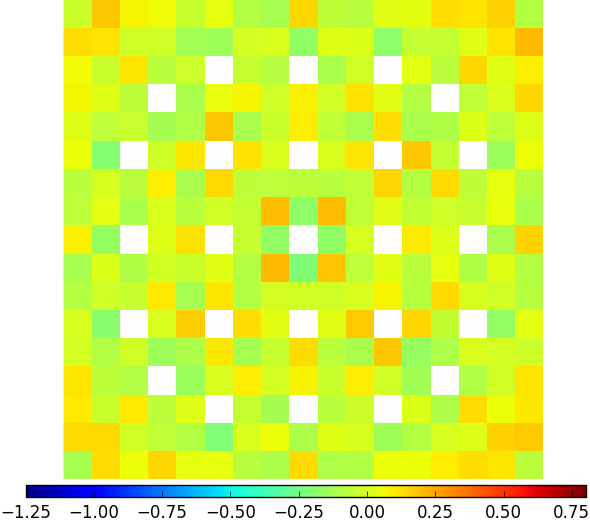
\includegraphics[width=\linewidth]{figures/results/assm-31/pca-transform/capt-err-lns}
  \caption{}
  \label{fig:chap11-assm-3.1-capt-lns}
\end{subfigure}%
\begin{subfigure}{0.45\textwidth}
  \centering
  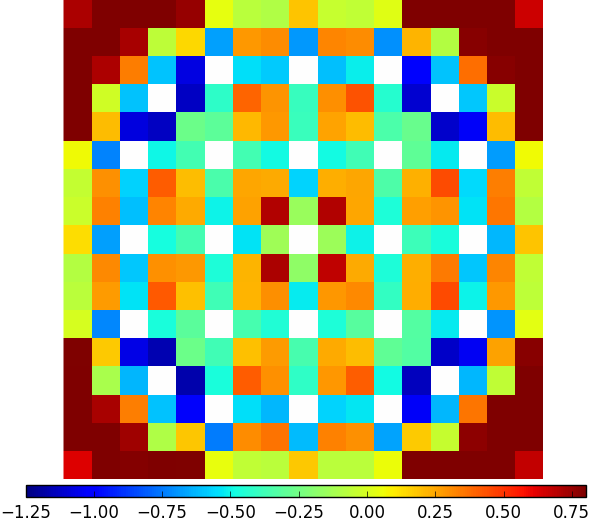
\includegraphics[width=\linewidth]{figures/results/assm-31/pca-transform/capt-err-pinch-agglomerative-(2)}
  \caption{}
  \label{fig:chap11-assm-3.1-capt-pinch-2}
\end{subfigure}
\begin{subfigure}{0.45\textwidth}
  \centering
  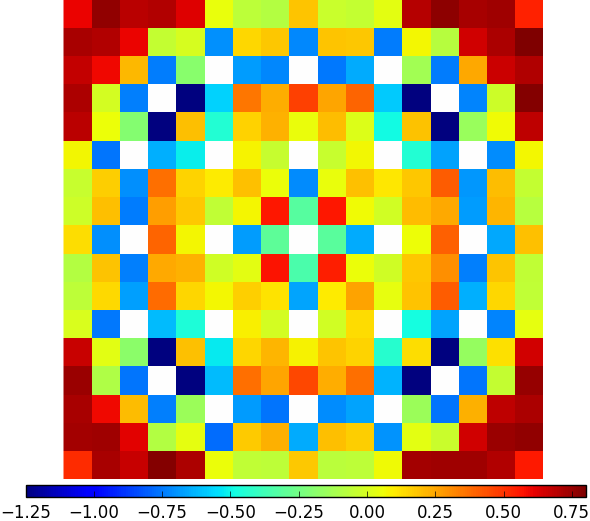
\includegraphics[width=\linewidth]{figures/results/assm-31/pca-transform/capt-err-pinch-agglomerative-(6)}
  \caption{}
  \label{fig:chap11-assm-3.1-capt-pinch-6}
\end{subfigure}%
\begin{subfigure}{0.45\textwidth}
  \centering
  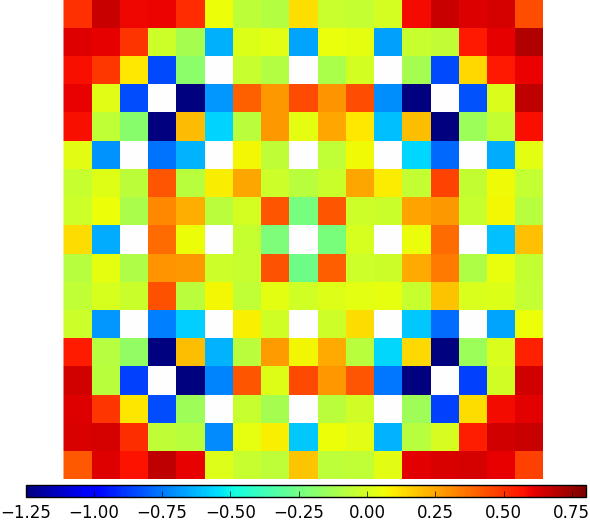
\includegraphics[width=\linewidth]{figures/results/assm-31/pca-transform/capt-err-pinch-agglomerative-(10)}
  \caption{}
  \label{fig:chap11-assm-3.1-capt-pinch-10}
\end{subfigure}
\vspace{2mm}
\caption[U-238 capture rate errors for a 3.1\% enriched assembly]{U-238 capture rate error spatial distributions for a 3.1\% enriched assembly for null (a), degenerate (b), \ac{LNS} (c) and \textit{i}\ac{MGXS} spatial homogenization with 2 (d), 6 (e) and 10 (f) clusters.}
\label{fig:chap11-assm-3.1-capt-rates}
\end{figure}

\clearpage

\begin{figure}[h!]
\centering
\begin{subfigure}{0.45\textwidth}
  \centering
  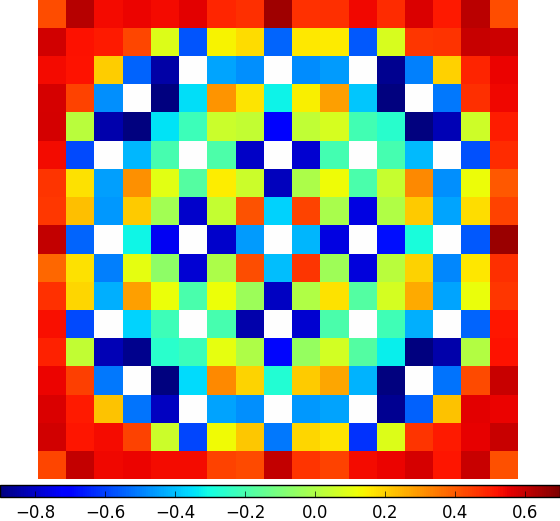
\includegraphics[width=\linewidth]{figures/results/assm-31-20BPs/no-transform/capt-err-null}
  \caption{}
  \label{fig:chap11-assm-3.1-20BPs-capt-null}
\end{subfigure}%
\begin{subfigure}{0.45\textwidth}
  \centering
  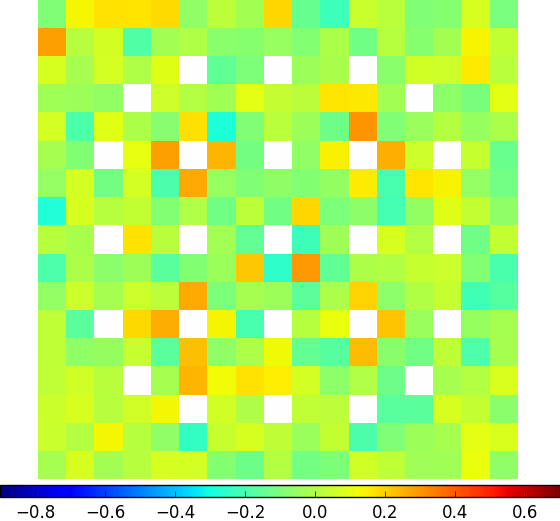
\includegraphics[width=\linewidth]{figures/results/assm-31-20BPs/no-transform/capt-err-degenerate}
  \caption{}
  \label{fig:chap11-assm-3.1-20BPs-capt-degenerate}
\end{subfigure}
\begin{subfigure}{0.45\textwidth}
  \centering
  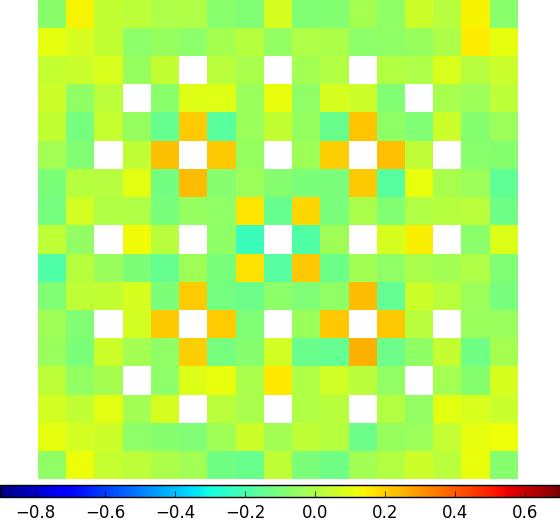
\includegraphics[width=\linewidth]{figures/results/assm-31-20BPs/no-transform/capt-err-lns}
  \caption{}
  \label{fig:chap11-assm-3.1-20BPs-capt-lns}
\end{subfigure}%
\begin{subfigure}{0.45\textwidth}
  \centering
  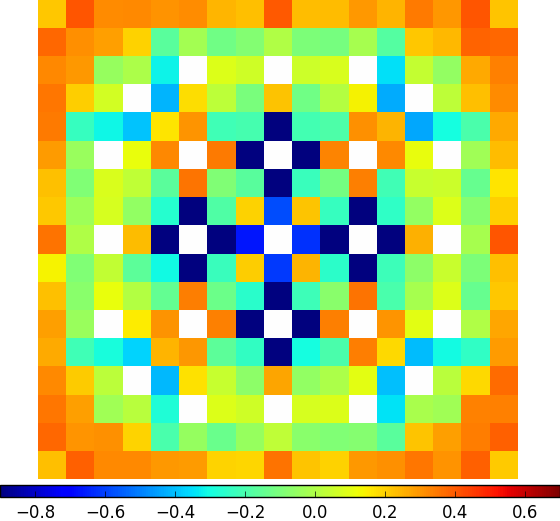
\includegraphics[width=\linewidth]{figures/results/assm-31-20BPs/no-transform/capt-err-pinch-agglomerative-(2)}
  \caption{}
  \label{fig:chap11-assm-3.1-20BPs-capt-pinch-2}
\end{subfigure}
\begin{subfigure}{0.45\textwidth}
  \centering
  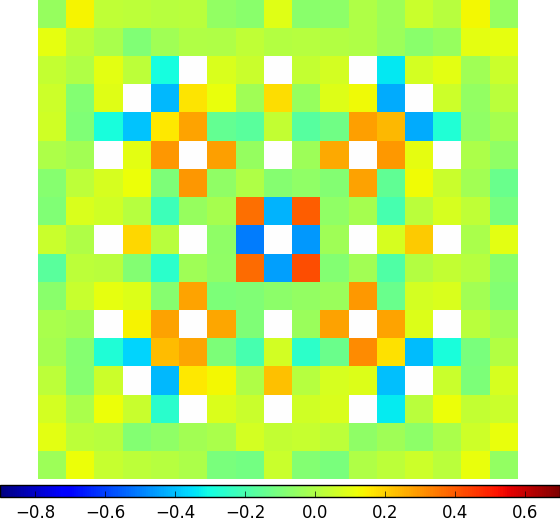
\includegraphics[width=\linewidth]{figures/results/assm-31-20BPs/no-transform/capt-err-pinch-agglomerative-(6)}
  \caption{}
  \label{fig:chap11-assm-3.1-20BPs-capt-pinch-6}
\end{subfigure}%
\begin{subfigure}{0.45\textwidth}
  \centering
  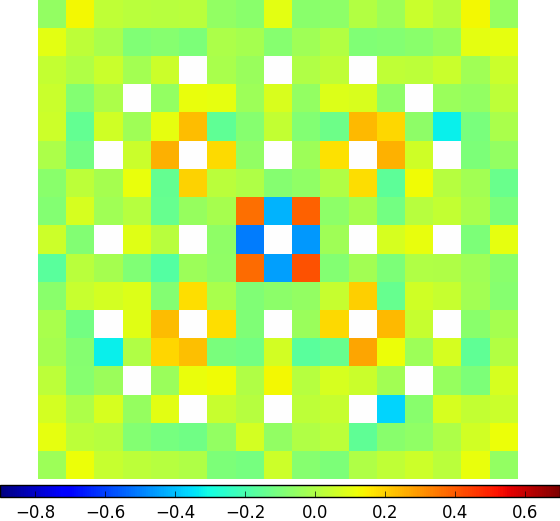
\includegraphics[width=\linewidth]{figures/results/assm-31-20BPs/no-transform/capt-err-pinch-agglomerative-(10)}
  \caption{}
  \label{fig:chap11-assm-3.1-20BPs-capt-pinch-10}
\end{subfigure}
\vspace{2mm}
\caption[U-238 capture rate errors for a 3.1\% enriched assembly with 20 BPs]{U-238 capture rate error spatial distributions for a 3.1\% enriched assembly with 20 \acp{BP} for null (a), degenerate (b), \ac{LNS} (c) and \textit{i}\ac{MGXS} spatial homogenization with 2 (d), 6 (e) and 10 (f) clusters.}
\label{fig:chap11-assm-3.1-20BPs-capt-rates}
\end{figure}

\clearpage

\begin{figure}[h!]
\centering
\begin{subfigure}{0.45\textwidth}
  \centering
  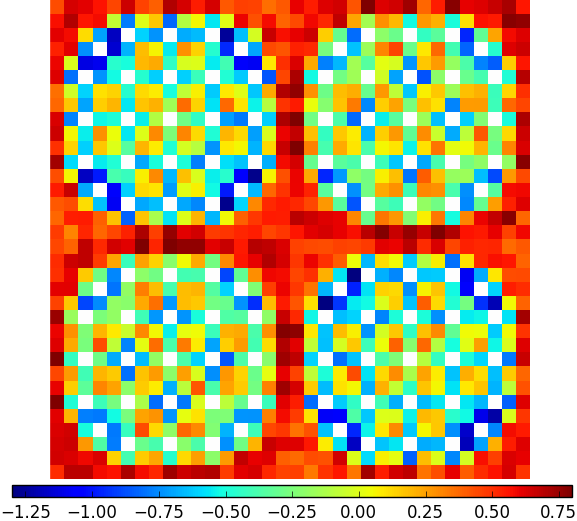
\includegraphics[width=\linewidth]{figures/results/2x2/ensemble-transform/capt-err-null}
  \caption{}
  \label{fig:chap11-assm-2x2-capt-null}
\end{subfigure}%
\begin{subfigure}{0.45\textwidth}
  \centering
  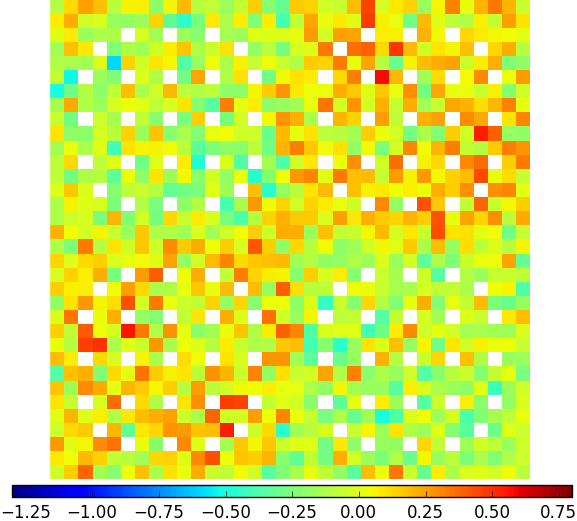
\includegraphics[width=\linewidth]{figures/results/2x2/ensemble-transform/capt-err-degenerate}
  \caption{}
  \label{fig:chap11-assm-2x2-capt-degenerate}
\end{subfigure}
\begin{subfigure}{0.45\textwidth}
  \centering
  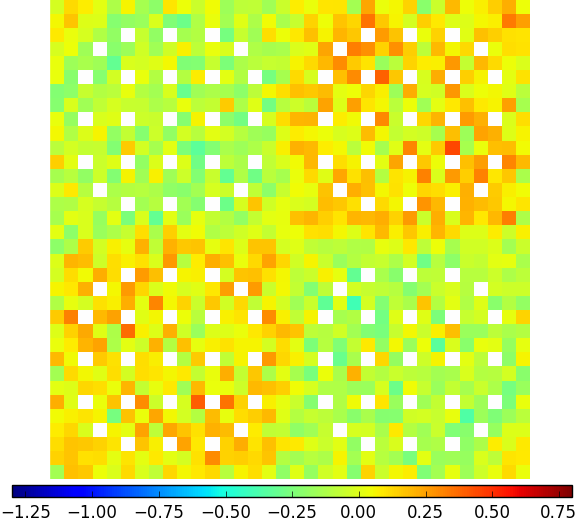
\includegraphics[width=\linewidth]{figures/results/2x2/ensemble-transform/capt-err-lns}
  \caption{}
  \label{fig:chap11-assm-2x2-capt-lns}
\end{subfigure}%
\begin{subfigure}{0.45\textwidth}
  \centering
  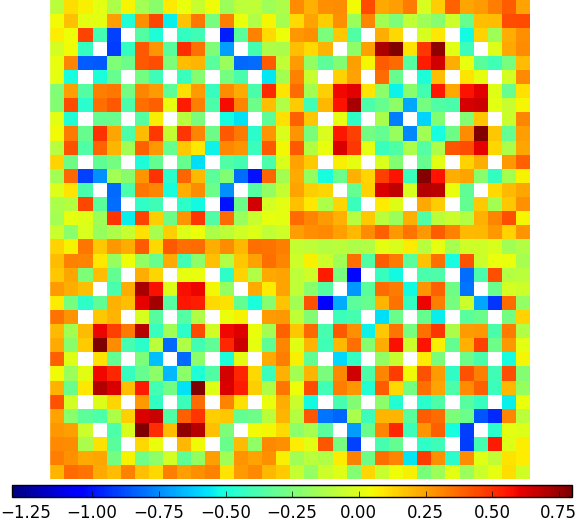
\includegraphics[width=\linewidth]{figures/results/2x2/ensemble-transform/capt-err-pinch-agglomerative-(2)}
  \caption{}
  \label{fig:chap11-assm-2x2-capt-pinch-2}
\end{subfigure}
\begin{subfigure}{0.45\textwidth}
  \centering
  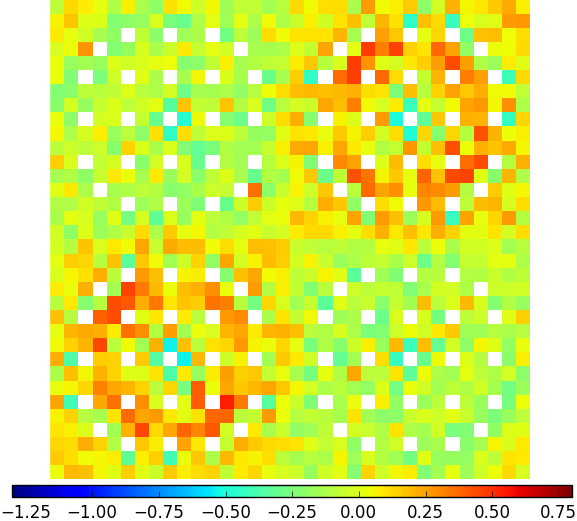
\includegraphics[width=\linewidth]{figures/results/2x2/ensemble-transform/capt-err-pinch-agglomerative-(6)}
  \caption{}
  \label{fig:chap11-assm-2x2-capt-pinch-6}
\end{subfigure}%
\begin{subfigure}{0.45\textwidth}
  \centering
  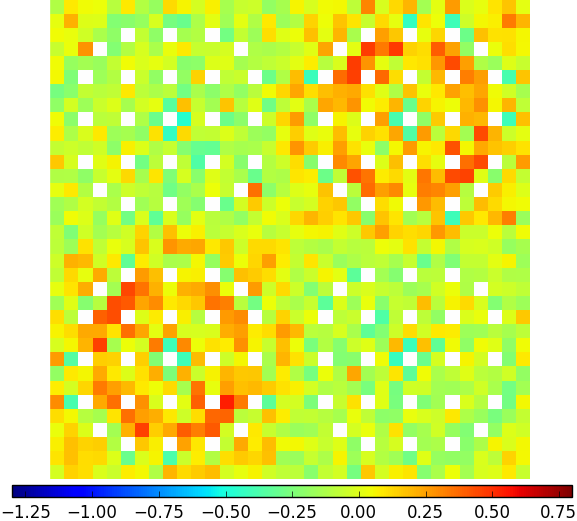
\includegraphics[width=\linewidth]{figures/results/2x2/ensemble-transform/capt-err-pinch-agglomerative-(10)}
  \caption{}
  \label{fig:chap11-assm-2x2-capt-pinch-10}
\end{subfigure}
\vspace{2mm}
\caption[U-238 capture rate errors for a 2$\times$2 colorset]{U-238 capture rate error spatial distributions for a 2$\times$2 colorset for null (a), degenerate (b), \ac{LNS} (c) and \textit{i}\ac{MGXS} spatial homogenization with 2 (d), 6 (e) and 10 (f) clusters.}
\label{fig:chap11-assm-2x2-capt-rates}
\end{figure}

\clearpage


%%%%%%%%%%%%%%%%%%%%%%%%%%%%%%%%%%%%%%%%%%%%%%%%%%%%%%%%%%%%%%%%%%%%%%%%%%%%%%%
\section{Convergence Rates}
\label{sec:chap11-convergence}

%%%%%%%%%%%%%%%%%%%%%%%%%%%%%%%%%%%
\subsection{Eigenvalue Convergence}
\label{subsec:chap11-eigenvalue-converge}

\clearpage

\begin{figure}[h!]
\centering
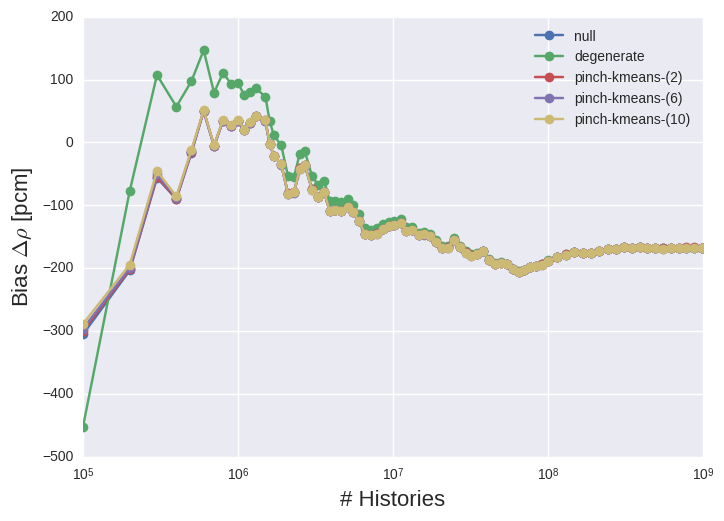
\includegraphics[width=0.85\linewidth]{figures/results/assm-16/no-transform/keff-bias}
\vspace{2mm}
\caption[Eigenvalue bias covergence for a 1.6\% enriched assembly]{Convergence of the eigenvalue bias $\Delta\rho$ for a 1.6\% enriched assembly for varying spatial homogenization schemes.}
\label{fig:chap11-assm-1.6-eigenvalue-converge}
\end{figure}

\begin{figure}[h!]
\centering
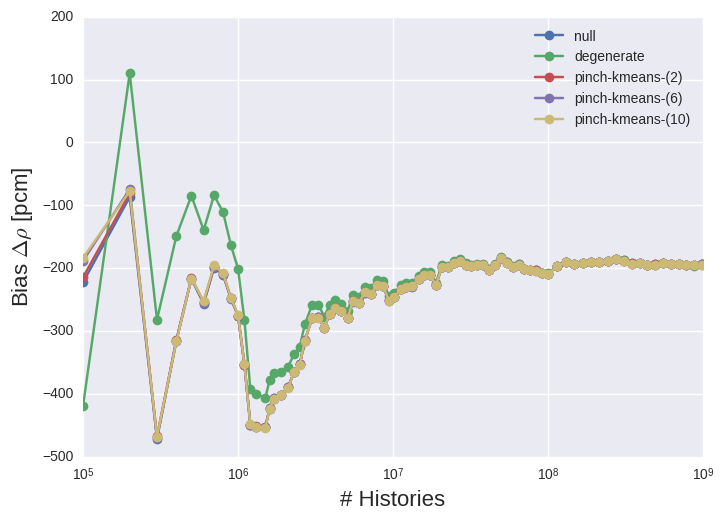
\includegraphics[width=0.85\linewidth]{figures/results/assm-31/pca-transform/keff-bias}
\vspace{2mm}
\caption[Eigenvalue bias covergence for a 3.1\% enriched assembly]{Convergence of the eigenvalue bias $\Delta\rho$ for a 3.1\% enriched assembly for varying spatial homogenization schemes.}
\label{fig:chap11-assm-3.1-eigenvalue-converge}
\end{figure}

\clearpage

\begin{figure}[h!]
\centering
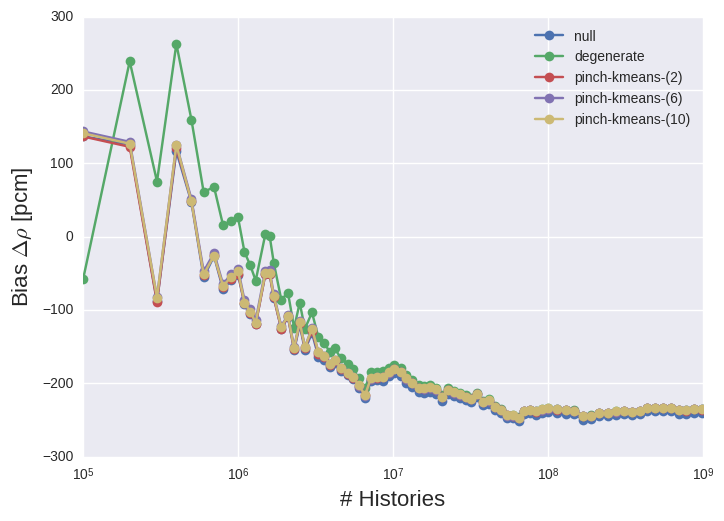
\includegraphics[width=0.85\linewidth]{figures/results/assm-31-20BPs/no-transform/keff-bias}
\vspace{2mm}
\caption[Eigenvalue bias covergence for a 3.1\% enriched assembly with 20 \acp{BP}]{Convergnce of the eigenvalue bias $\Delta\rho$ for a 3.1\% enriched assembly with 20 \acp{BP} for varying spatial homogenization schemes.}
\label{fig:chap11-assm-3.1-20BPs-eigenvalue-converge}
\end{figure}

\begin{figure}[h!]
\centering
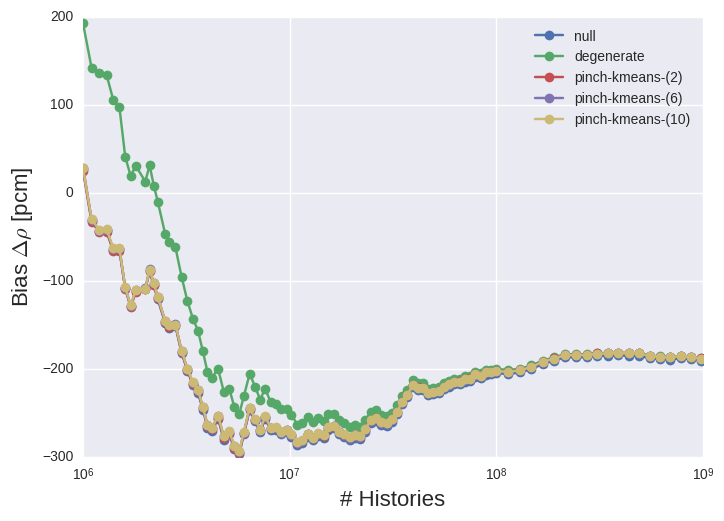
\includegraphics[width=0.85\linewidth]{figures/results/2x2/ensemble-transform/keff-bias}
\vspace{2mm}
\caption[Eigenvalue bias covergence for a 2$\times$2 colorset]{Convergnce of the eigenvalue bias $\Delta\rho$ for a 2$\times$2 colorset for varying spatial homogenization schemes.}
\label{fig:chap11-2x2-eigenvalue-converge}
\end{figure}

\clearpage


%%%%%%%%%%%%%%%%%%%%%%%%%%%%%%%%%%%%%
\subsection{Fission Rate Convergence}
\label{subsec:chap11-fission-converge}

\clearpage

\begin{figure}[h!]
\centering
\begin{subfigure}{\textwidth}
  \centering
  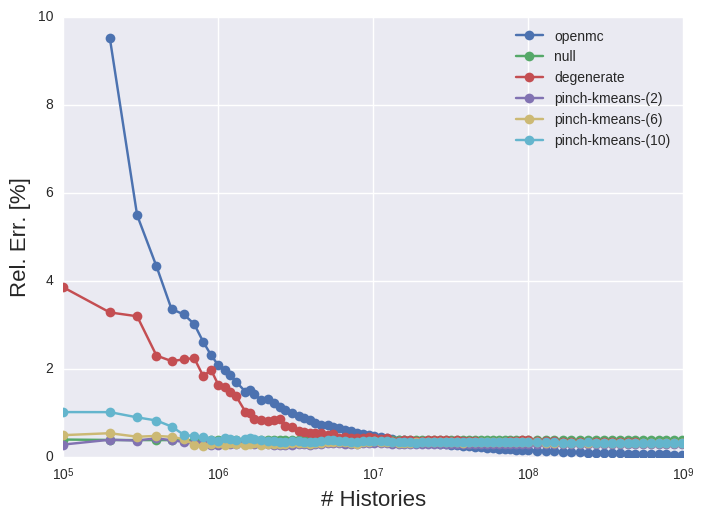
\includegraphics[width=0.9\linewidth]{figures/results/assm-16/no-transform/evo-fission-max}
  \caption{}
  \label{fig:chap11-assm-1.6-fission-converge-max}
\end{subfigure}
\begin{subfigure}{\textwidth}
  \centering
  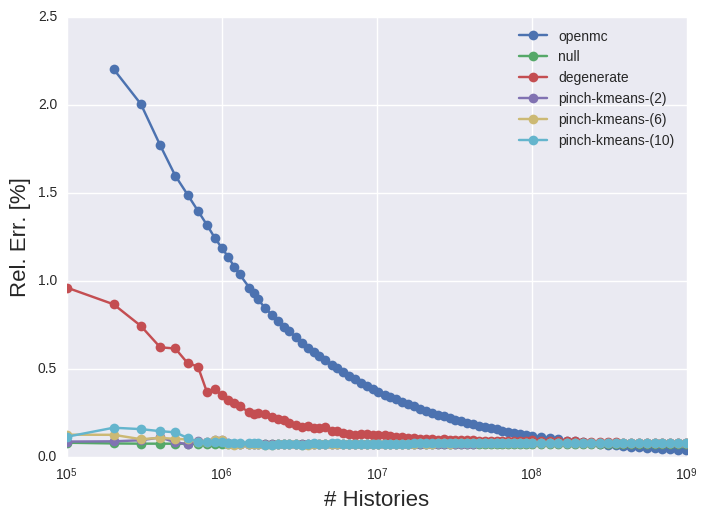
\includegraphics[width=0.9\linewidth]{figures/results/assm-16/no-transform/evo-fission-mean}
  \caption{}
  \label{fig:chap11-assm-1.6-fission-converge-mean}
\end{subfigure}
\vspace{2mm}
\caption[Fission rate covergence for a 1.6\% enriched assembly]{Convergence of the max (a) and mean (b) absolute fission rate percent relative errors for a 1.6\% enriched assembly for varying spatial homogenization schemes.}
\label{fig:chap11-assm-1.6-fission-converge}
\end{figure}

\clearpage

\begin{figure}[h!]
\centering
\begin{subfigure}{\textwidth}
  \centering
  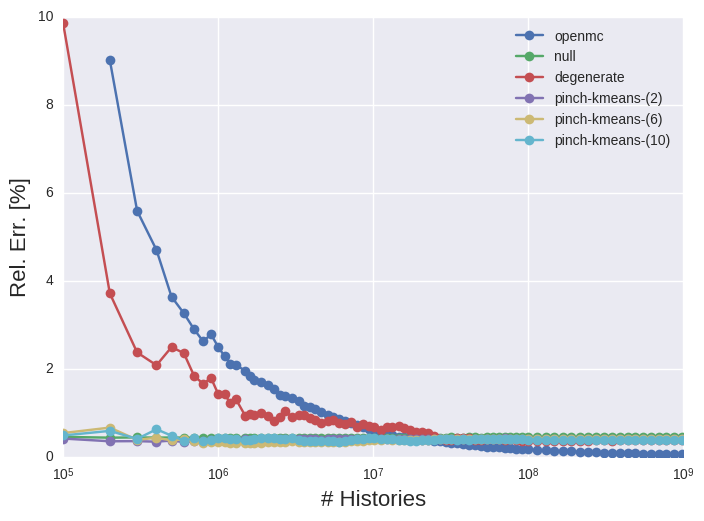
\includegraphics[width=0.9\linewidth]{figures/results/assm-31/pca-transform/evo-fission-max}
  \caption{}
  \label{fig:chap11-assm-3.1-fission-converge-max}
\end{subfigure}
\begin{subfigure}{\textwidth}
  \centering
  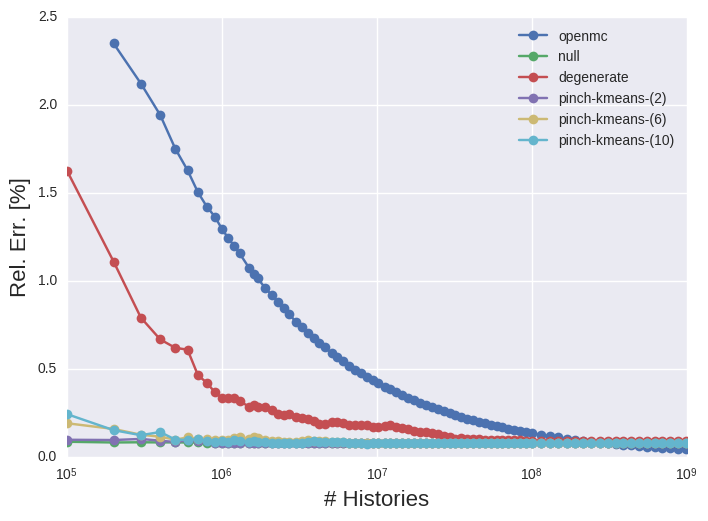
\includegraphics[width=0.9\linewidth]{figures/results/assm-31/pca-transform/evo-fission-mean}
  \caption{}
  \label{fig:chap11-assm-3.1-fission-converge-mean}
\end{subfigure}
\vspace{2mm}
\caption[Fission rate covergence for a 3.1\% enriched assembly]{Convergence of the max (a) and mean (b) absolute fission rate percent relative errors for a 3.1\% enriched assembly for varying spatial homogenization schemes.}
\label{fig:chap11-assm-3.1-fission-converge}
\end{figure}

\clearpage

\begin{figure}[h!]
\centering
\begin{subfigure}{\textwidth}
  \centering
  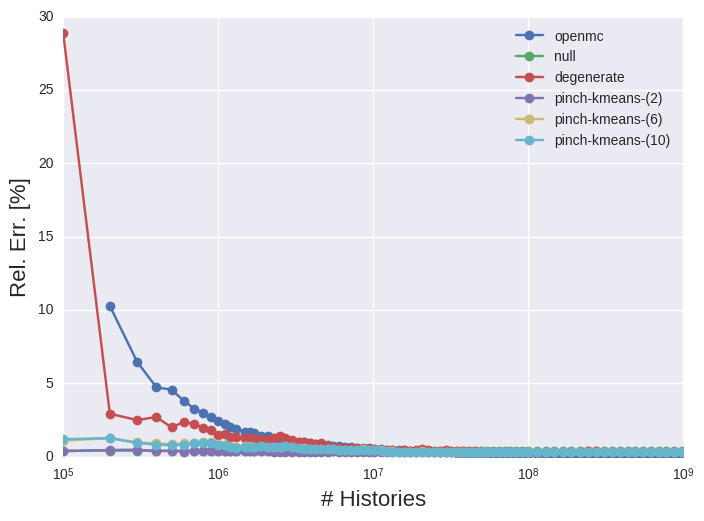
\includegraphics[width=0.9\linewidth]{figures/results/assm-31-20BPs/no-transform/evo-fission-max}
  \caption{}
  \label{fig:chap11-assm-3.1-20BPs-fission-converge-max}
\end{subfigure}
\begin{subfigure}{\textwidth}
  \centering
  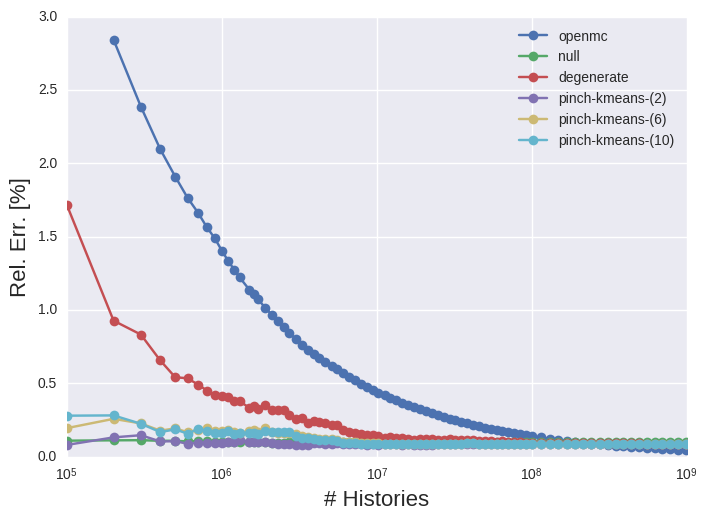
\includegraphics[width=0.9\linewidth]{figures/results/assm-31-20BPs/no-transform/evo-fission-mean}
  \caption{}
  \label{fig:chap11-assm-3.1-20BPs-fission-converge-mean}
\end{subfigure}
\vspace{2mm}
\caption[Fission rate covergence for a 3.1\% enriched assembly with 20 \acp{BP}]{Convergence of the max (a) and mean (b) absolute fission rate percent relative errors for a 3.1\% enriched assembly with 20 \acp{BP} for varying spatial homogenization schemes.}
\label{fig:chap11-assm-3.1-20BPs-fission-converge}
\end{figure}

\clearpage

\begin{figure}[h!]
\centering
\begin{subfigure}{\textwidth}
  \centering
  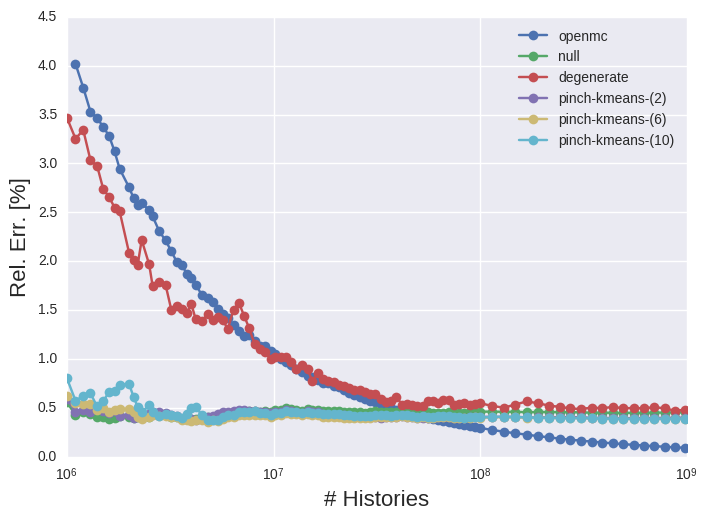
\includegraphics[width=0.9\linewidth]{figures/results/2x2/ensemble-transform/evo-fission-max}
  \caption{}
  \label{fig:chap11-2x2-fission-converge-max}
\end{subfigure}
\begin{subfigure}{\textwidth}
  \centering
  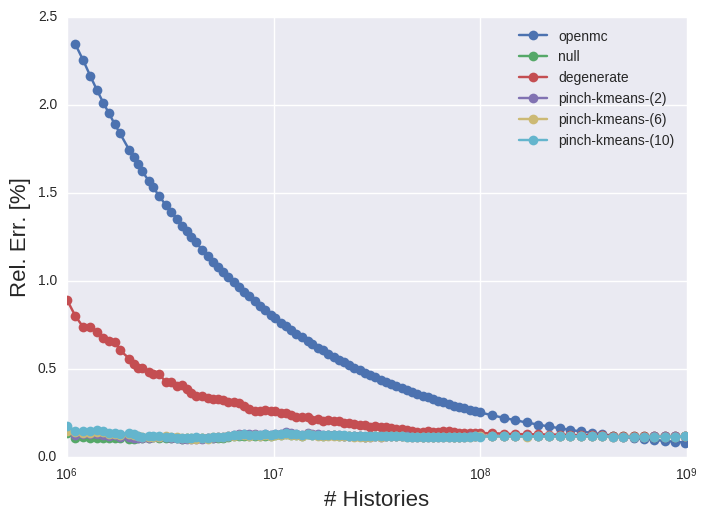
\includegraphics[width=0.9\linewidth]{figures/results/2x2/ensemble-transform/evo-fission-mean}
  \caption{}
  \label{fig:chap11-2x2-fission-converge-mean}
\end{subfigure}
\vspace{2mm}
\caption[Fission rate covergence for a 2$\times$2 colorset]{Convergence of the max (a) and mean (b) absolute fission rate percent relative errors for a 2$\times$2 colorset for varying spatial homogenization schemes.}
\label{fig:chap11-2x2-fission-converge}
\end{figure}

\clearpage

%%%%%%%%%%%%%%%%%%%%%%%%%%%%%%%%%%%%%%%%%%%
\subsection{U-238 Capture Rate Convergence}
\label{subsec:chap11-capture-converge}

\clearpage

\begin{figure}[h!]
\centering
\begin{subfigure}{\textwidth}
  \centering
  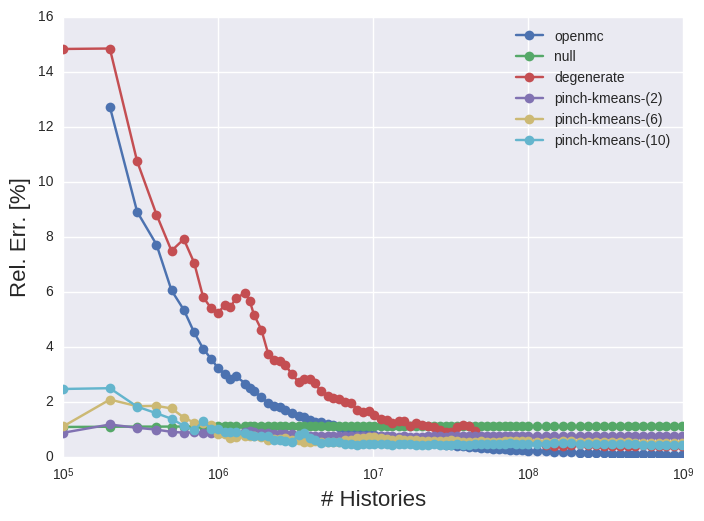
\includegraphics[width=0.9\linewidth]{figures/results/assm-16/no-transform/evo-capture-max}
  \caption{}
  \label{fig:chap11-assm-1.6-capture-converge-max}
\end{subfigure}
\begin{subfigure}{\textwidth}
  \centering
  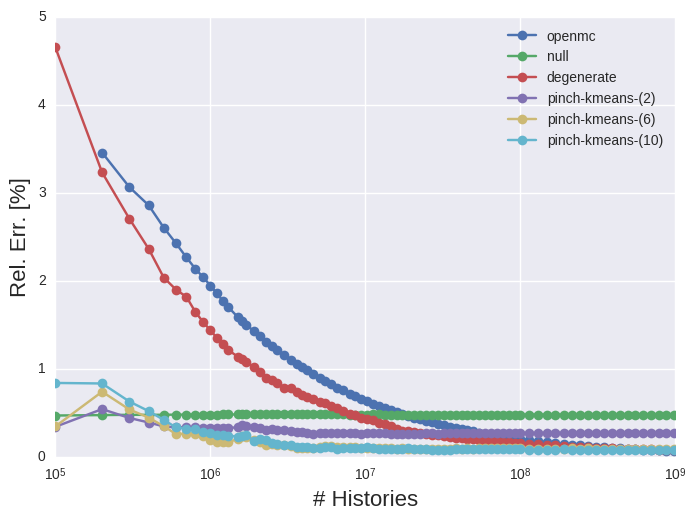
\includegraphics[width=0.9\linewidth]{figures/results/assm-16/no-transform/evo-capture-mean}
  \caption{}
  \label{fig:chap11-assm-1.6-capture-converge-mean}
\end{subfigure}
\vspace{2mm}
\caption[Fission rate covergence for a 1.6\% enriched assembly]{Convergence of the max (a) and mean (b) absolute U-238 capture rate percent relative errors for a 1.6\% enriched assembly for varying spatial homogenization schemes.}
\label{fig:chap11-assm-1.6-capture-converge}
\end{figure}

\clearpage

\begin{figure}[h!]
\centering
\begin{subfigure}{\textwidth}
  \centering
  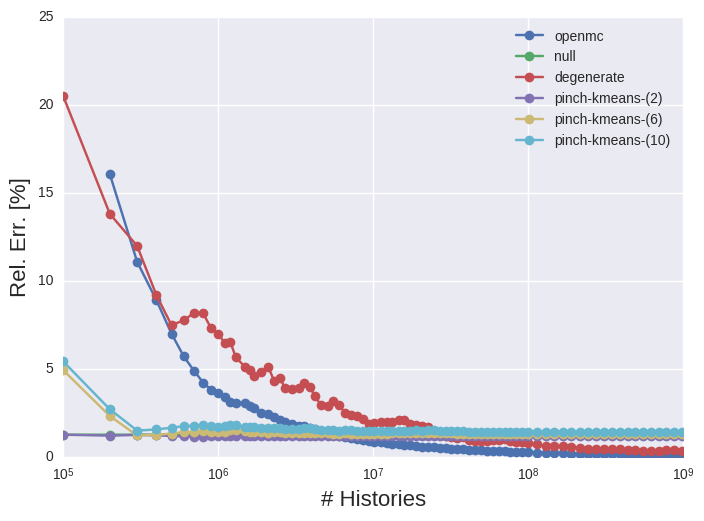
\includegraphics[width=0.9\linewidth]{figures/results/assm-31/pca-transform/evo-capture-max}
  \caption{}
  \label{fig:chap11-assm-3.1-capture-converge-max}
\end{subfigure}
\begin{subfigure}{\textwidth}
  \centering
  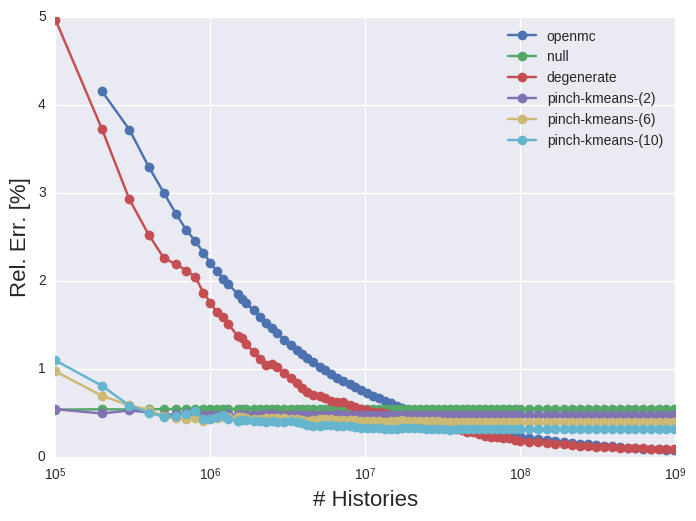
\includegraphics[width=0.9\linewidth]{figures/results/assm-31/pca-transform/evo-capture-mean}
  \caption{}
  \label{fig:chap11-assm-3.1-capture-converge-mean}
\end{subfigure}
\vspace{2mm}
\caption[Fission rate covergence for a 3.1\% enriched assembly]{Convergence of the max (a) and mean (b) absolute U-238 capture rate percent relative errors for a 3.1\% enriched assembly for varying spatial homogenization schemes.}
\label{fig:chap11-assm-3.1-capture-converge}
\end{figure}

\clearpage

\begin{figure}[h!]
\centering
\begin{subfigure}{\textwidth}
  \centering
  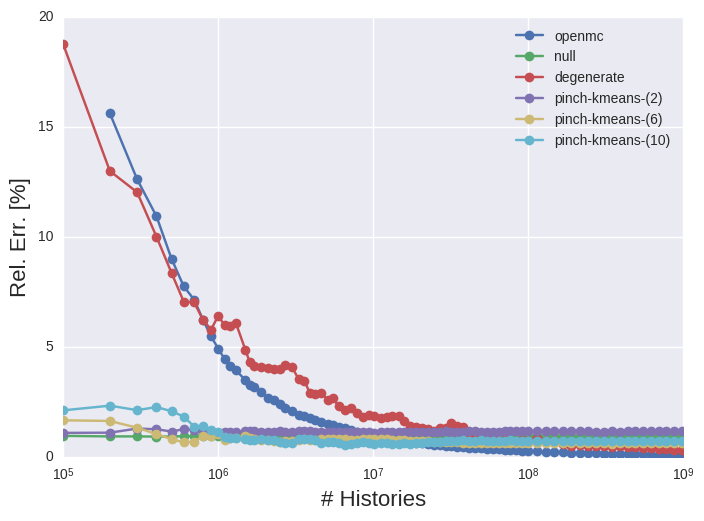
\includegraphics[width=0.9\linewidth]{figures/results/assm-31-20BPs/no-transform/evo-capture-max}
  \caption{}
  \label{fig:chap11-assm-3.1-20BPs-capture-converge-max}
\end{subfigure}
\begin{subfigure}{\textwidth}
  \centering
  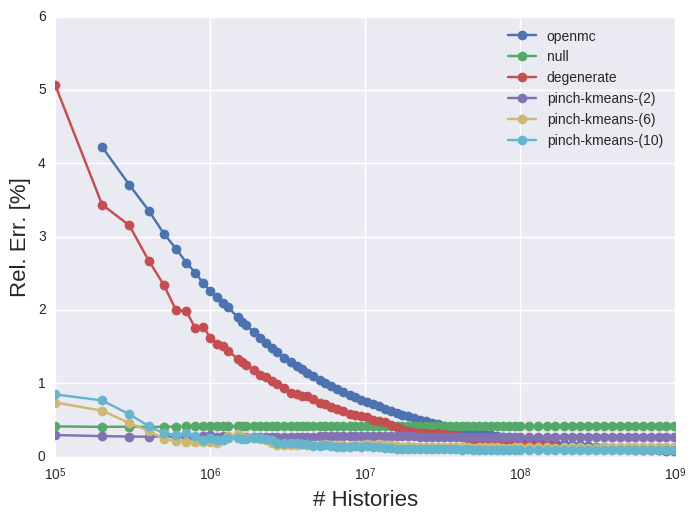
\includegraphics[width=0.9\linewidth]{figures/results/assm-31-20BPs/no-transform/evo-capture-mean}
  \caption{}
  \label{fig:chap11-assm-3.1-20BPs-capture-converge-mean}
\end{subfigure}
\vspace{2mm}
\caption[Fission rate covergence for a 3.1\% enriched assembly with 20 \acp{BP}]{Convergence of the max (a) and mean (b) absolute U-238 capture rate percent relative errors for a 3.1\% enriched assembly with 20 \acp{BP} for varying spatial homogenization schemes.}
\label{fig:chap11-assm-3.1-20BPs-capture-converge}
\end{figure}

\clearpage

\begin{figure}[h!]
\centering
\begin{subfigure}{\textwidth}
  \centering
  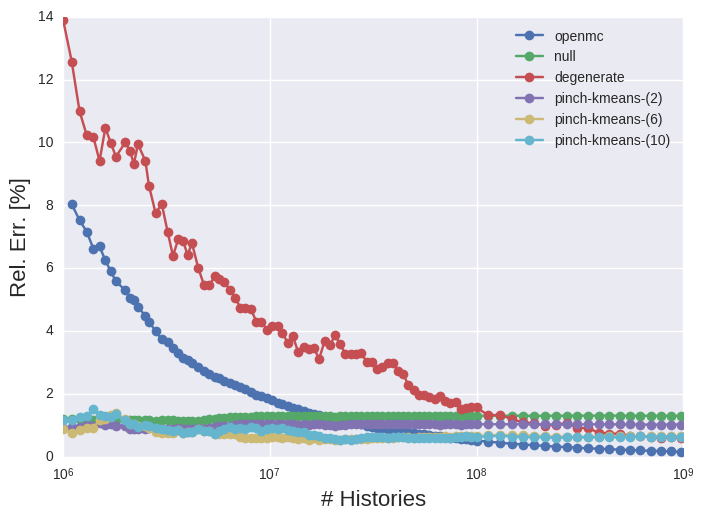
\includegraphics[width=0.9\linewidth]{figures/results/2x2/ensemble-transform/evo-capture-max}
  \caption{}
  \label{fig:chap11-2x2-capture-converge-max}
\end{subfigure}
\begin{subfigure}{\textwidth}
  \centering
  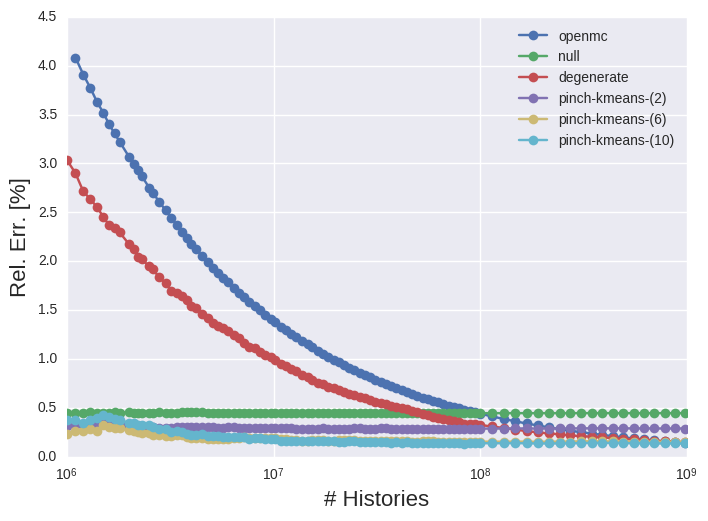
\includegraphics[width=0.9\linewidth]{figures/results/2x2/ensemble-transform/evo-capture-mean}
  \caption{}
  \label{fig:chap11-2x2-capture-converge-mean}
\end{subfigure}
\vspace{2mm}
\caption[Fission rate covergence for a 2$\times$2 colorset]{Convergence of the max (a) and mean (b) absolute U-238 capture rate percent relative errors for a 2$\times$2 colorset for varying spatial homogenization schemes.}
\label{fig:chap11-2x2-capture-converge}
\end{figure}

\clearpage
